\documentclass[12pt]{article}
\usepackage{graphicx}
\usepackage{fullpage}
\usepackage{float}
\usepackage[symbol]{footmisc}
\graphicspath{{../images/}}

\title {Astron 121: Analog Lab}
\author {
Kevin Yu
}

\begin{document}
\maketitle

\begin{abstract}
We study the properties of basic analog circuit components, and demonstrate how they can be used to filter and manipulate electrical signals. Our study of manipulating signals culminated in the construction of an FM receiver capable of demodulating and amplifying an incoming signal carried at $1.045MHz$. Additionally, we use our powerful new understanding of impedances and reflections due to impedance mismatches to estimate the length of a long cable. We measure the cable to be roughly ~$120m$, and the characteristic impedance of the cable to be about $56\Omega$. Finally, we study possible sources and characteristics of noise in analog circuits; we measure the noise factor (NF) of our circuit to be $TODO \pm TODO$ LOL. To learn how to characterize noise, we empirically verify the Central Limit Theorem (CLT), finding that the standard deviation of the sample average of $n$ measurements is proportional to $n^{-0.51\pm0.02}$, in agreement with the CLT prediction of $\sigma \propto n^{-0.5}$.
\end{abstract}

\section*{Introduction}
In this first lab, we will begin to understand how to understand and manipulate radio signals using analog circuits. Understanding the basics of impedances will help us build frequency dependent filters so that we can extract the information we want from signals while excluding superfluous noise and offsets. We will learn the importance of impedance matching, both between circuit components, where a mismatch in impedances can cause one section of the circuit to significantly alter the behavior of another, as well as impedance matching in transmission lines, where a mismatch can result in distortive effects due to reflections.

We will demonstrate these tools immediately by building a FM Receiver, which will take an FM signal and convert it into a signal that we can listen to on a speaker. This will take advantage of LC and RC filters, DC biasing, and using NPN transistors to help us amplify our signal. We will learn optimization techniques such as proper termination, as well as ways we can characterize random noise in our results. Also we will learn how to write lab reports in a semi-professional and non-sarcastic manner.

\section*{Theory}

\subsection*{Impedance}
Impedance is a generalization of resistance that, through Ohm's Law $V=IR$, relates the current through a component to the voltage across it. In the case of capacitors and inductors, impedances can be both complex and frequency dependent. The impedances of resistors, capacitors, and inductors are:
\begin{eqnarray}
Z_{resistor} &=& R\nonumber\\
Z_{capacitor} &=& (j\omega C)^{-1} \nonumber \\
Z_{inductor} &=& j\omega L \nonumber
\end{eqnarray}
As you can see, capacitors have high impedances for low-frequency and DC signals, but have little impedance for high-frequency signals. Conversely, inductors oppose high-frequency signals while pass through low-frequency and DC signals.

Impedances add in the same way that resistances do.
\begin{eqnarray}
Z_{series} &=& \sum_i{Z_i}\nonumber\\
\frac{1}{Z_{parallel}} &=& \sum_i{\frac{1}{Z_i}}\nonumber
\end{eqnarray}

As an example of adding frequency dependent and complex impedances, Fig.\ref{fig:LCimpedances} shows the impedance of an inductor and capacitor combined at different frequencies.
\begin{figure}[H]
\center{
  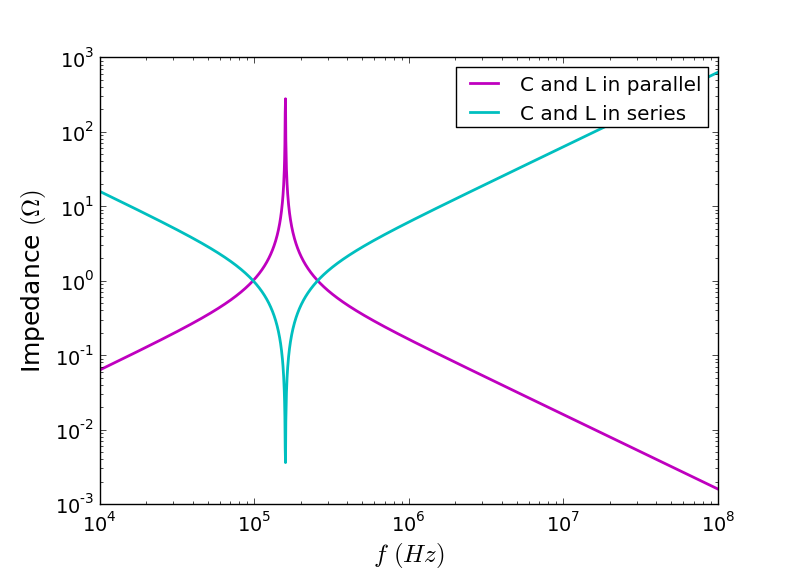
\includegraphics[width=360px]{LC_parallel_series}
}
\caption{Impedance of an inductor and a capacitor connected in parallel and in series. At the frequency $\omega_0=\frac{1}{\sqrt{LC}}$, the impedance of the two in series goes to zero, while the impedance of the two in parallel becomes infinitely large (this is at the LC circuit's resonant frequency).}
\label{fig:LCimpedances}
\end{figure}

\subsection*{Reflections and Termination}
At the interface between two conductors with different impedances, a signal can be partially, or entirely, reflected back from whence it came. When a signal reaches an interface going from a low impedance conductor to a high impedance conductor, the signal will be reflected with no inversion. At an interface from a high impedance conductor to a lower impedance conductor, the signal will be reflected and inverted. If the time delay between the a signal and its reflection is measured, the length of the cable can be approximated by the simple formula\footnote{Approximating the speed of signal propogation in the cable to be $\frac{2}{3}c$}:

\begin{eqnarray}
l_{cable} = \frac{2c}{3} \frac{\Delta{t}_{delay}}{2} \label{eq:cablelength}
\end{eqnarray}

To get rid of reflections, which can distort a signal, the cables should be properly terminated with an impedance matching the characteristic impedance of the cable itself, which will minimize unwanted reflections.

\subsection*{Voltage Divider}
A basic use of impedances is the voltage divider. A voltage divider, depicted in Fig.\ref{fig:voltagedivider}, obeys the following relationship, which can be derived directly from Ohm's law, $V=IZ$.
\begin{eqnarray}
V_{out} = \frac{Z_2}{Z_1+Z_2} V_{in} \label{eq:voltagedivider}
\end{eqnarray}
\begin{figure}[H]
\center{
  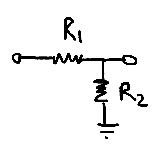
\includegraphics{volt_divider}
}
\caption{Voltage divider, shamelessly stolen from the lab manual.}
\label{fig:voltagedivider}
\end{figure}

\subsection*{RC Filter}
One application of a voltage divider is an RC filter. An RC filter is a voltage divider consisting of a resistor and a capacitor. A high-pass filter involves a capacitor connecting input to output and a resistor connecting output to ground; in Eq.\ref{eq:voltagedivider}, it corresponds to $Z_1=Z_C$ and $Z_2=R$. A high-pass filter lets through high frequency signals because for large $\omega$, $|Z_C| \ll |Z_R|$ and $Gain\footnote{Gain defined as $V_{out}/V_{in}$} \rightarrow 1$. For low frequency signals, $|Z_C| \gg |Z_R|$ and $Gain \rightarrow 0$, meaning the signal will be completely attenuated.

A low-pass filter is similar to the high-pass filter, with the positions of the capacitor and resistor reversed. Through similar arguments at high and low frequency limits, the gain goes to $1$ at low frequencies and goes to $0$ at high frequencies.

In both the high-pass and low-pass cases, there is a frequency at which the power output of the voltage divider is halved; i.e. $(V_{out}/V_{in})^2 = 0.5$ In decibels (dB)\footnote{decibels are defined as $20log_{10}{(V_{out}/V_{in})}$}, this is the $-3dB$ point. In RC filters, this occurs at the roll-off frequency
\begin{eqnarray}
\omega = \frac{1}{RC}\label{eq:rolloff}
\end{eqnarray}
A dramatic portrayal of the response of high-pass and low-pass filters can be seen in Fig.\ref{fig:highandlowpass}.
\begin{figure}[H]
\center{
  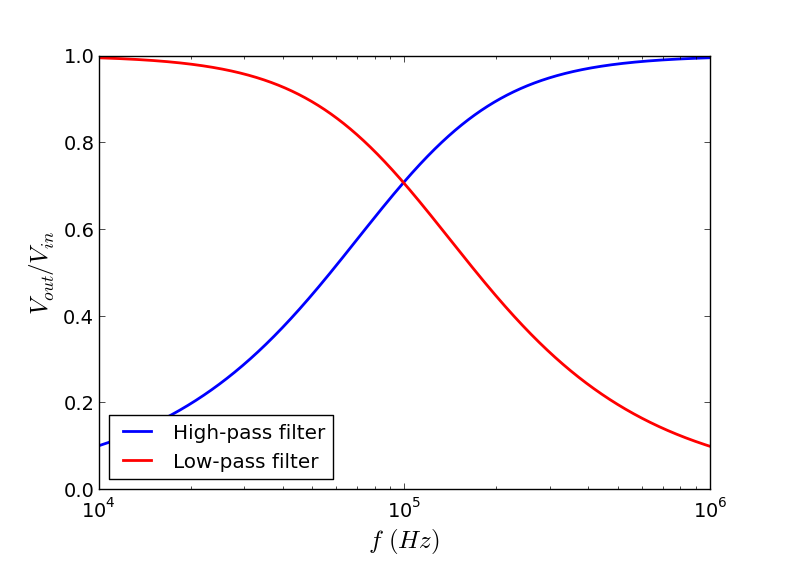
\includegraphics[width=360px]{RC_High_and_Low_pass}
}
\caption{Theoretical transfer functions for RC high-pass and low-pass filters with the same roll-off frequency of $10kHz$.}
\label{fig:highandlowpass}
\end{figure}
\subsection*{FM Demodulator}
We will be using the above to build a circuit capable of receiving a frequency-modulated (FM) signal and extracting the underlying signal. The modulated carrier wave will be a frequnecy a few orders of magnitude higher than the modulating signal. In this section I will describe how the demodulation works, referring to the circuit diagram in Fig.\ref{fig:fmdemoddiagram} for each separate section.
\begin{figure}[H]
\center{
  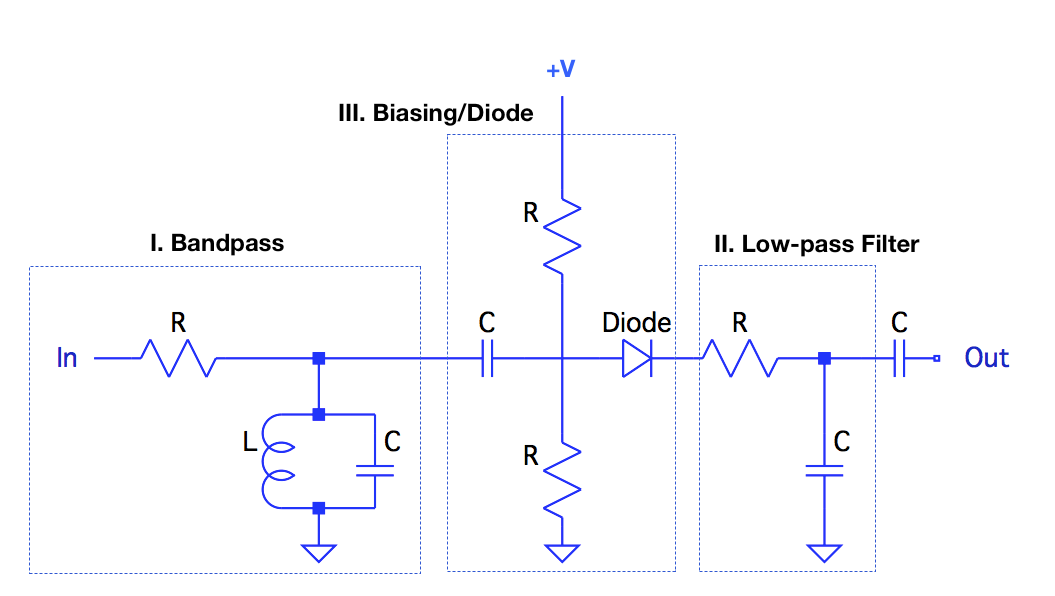
\includegraphics[width=360px]{fmdemod_diagram}
}
\caption{Depiction of the FM Demodulator.}
\label{fig:fmdemoddiagram}
\end{figure}

\subsection*{I. LC Bandpass Filter}
A capacitor and inductor can be combined in parallel to create a bandpass filter, a filter which only passes signals in a certain frequency range unattenuated. It is done by taking advantage of the behavior of an inductor and capacitor in parallel (Fig.\ref{fig:LCimpedances}). Near the resonant frequency of an LC loop,
\begin{eqnarray}
\omega_0 = \frac{1}{\sqrt{LC}} \label{eq:resonantfrequency}
\end{eqnarray}
The LC bandpass filter that we will create is a voltage divider with a resistor connecting the input and output, and an inductor and capacitor, in parallel, connecting the output to ground.

What this does is create an extremeley large $Z_2$ in Eq.\ref{eq:voltagedivider} at frequencies near the resonant frequency, leading to little attenuation, while having a small $Z_2$ farther from the resonant frequency, leading to significant attenuation. The end result is that only frequencies near the resonant frequency get passed through.

The resistor, $Z_1$ in this case, determines the bandwidth of the filter; it affects *how* far from resonance a signal must be before $Z_2 \approx Z_1$. The width of the bandpass can be defined in terms of the same $-3dB$ level of attenuation used in the earlier RC section:
\begin{eqnarray}
\Delta{f}_{-3dB} = \frac{f_0}{Q}\label{eq:bandwidth}\\
Q = R\sqrt{\frac{C}{L}}\nonumber
\end{eqnarray}

The purpose of this bandpass filter is to differentially attenuate frequencies in the FM modulation span. By tuning the resonant frequency of the bandpass to a value slightly below the center carrier frequency, and choosing the right $Q$, we can have the carrier wave's frequencies span the linear region (downward sloped) region of the bandpass filter's response. This can be seen in Fig.\ref{fig:bandpasstransfer}; higher frequency sections of this signal will have decreased amplitudes, thus converting the FM signal into an amplitude modulated (AM) signal.

\subsubsection*{II. Low-pass Filter}
Now we have an AM signal, and we want to remove the high frequency carrier wave, leaving only the lower frequency (audible frequency) signal behind. To do this, we can use a low-pass filter. Because the capacitor in the low-pass filter responds slowly to high frequency changes, by picking a filter with a roll-off below the carrier frequencies we can average out the carrier wave. However, we still want to preserve the amplitude information. Because the signal spends an equal amount of time below and above zero, the signal will be averaged out to zero and the amplitude information will be lost! To fix this, we will use a diode.

\subsubsection*{III. Biasing and Diode}
A diode is a component that only conducts current in one direction\footnote{unless the upstream voltage is greater than a certain critical value, which we should not encounter in this lab} if the voltage across it exceeds a critical value (in our case, it will be about $0.6V$). Once conducting, the voltage drop across the diode stays at a constant value until the signal drops back down below $0.6V$.

In the last section, we saw that we needed a way to preserve the amplitude information when smoothing over our signal. To do this, we will try only keep the positive half of the AM signal propogate, while blocking out the negative half. Instead of averaging out both positive and negative, which will zero out the signal, if we only average the positive half of the signal the low pass filter will smooth out the carrier frequency bumps but leave the relative amplitude information intact. To do this, we choose biasing resistors in the voltage divider such that Eq.\ref{eq:voltagedivider} gives us a biasing voltage of about $0.6V$. Note that the coupling capacitor right before the voltage divider ensures that there is no DC bias onther than the bias we provide here.

\subsection*{Amplifier}
TODO

\subsection*{Follower}
TODO

\subsection*{Noise}
\subsubsection*{Noise Factor}
TODO
\subsubsection*{Central Limit Theorem}
TODO

\section*{Method}

\subsection*{FM Receiver}
In this Lab, we will build an receiver tuned to a FM carrier frequency centered at $1.045MHz$.

\begin{figure}[H]
\center{
  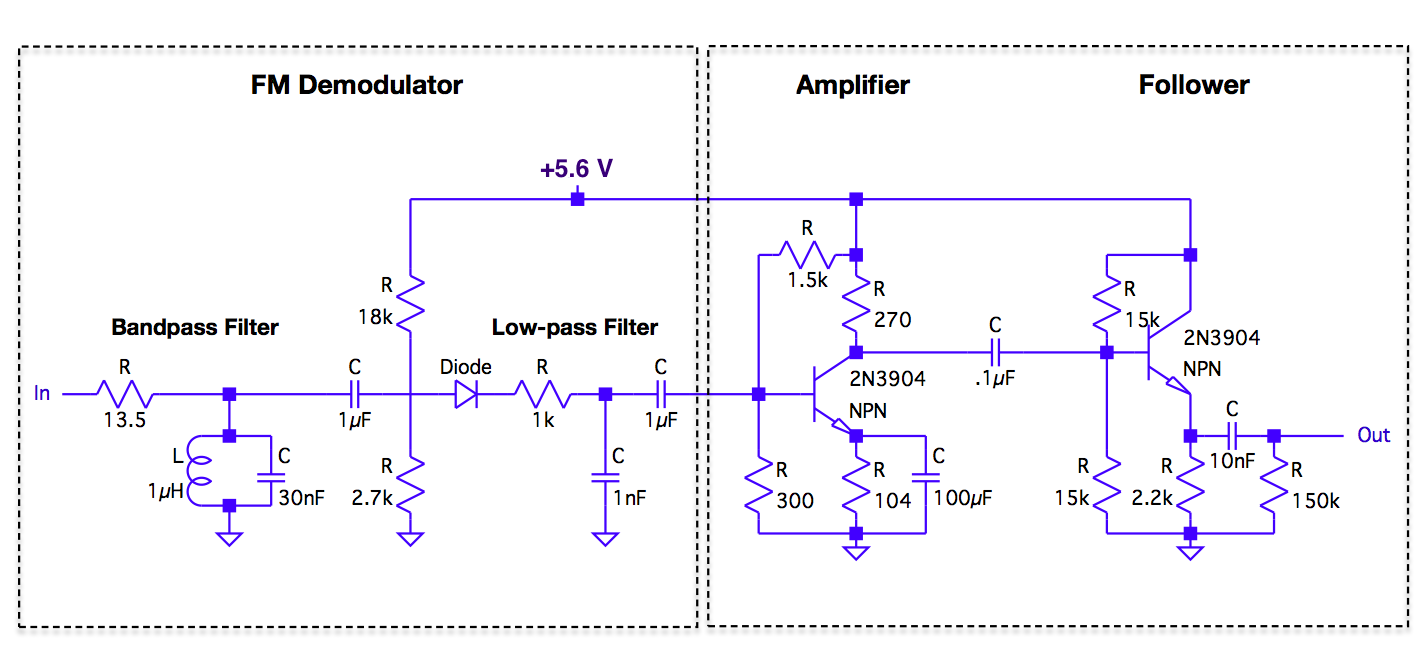
\includegraphics[width=480px]{Circuit_diagram_labeled_and_cropped}
}
\caption{Circuit diagram of our FM Receiver, with our selected component values. It consists of a FM demodulator connected in series with an amplifier and an emitter-follower.}
\label{fig:circuitdiagram}
\end{figure}

\subsubsection*{FM Demodulator}
The first part of the FM Demodulator is the bandpass filter. As we discussed in the earlier section, we want to tune our LC bandpass filter to be centered at a frequency slightly below the carrier frequency, and to choose a bandwidth that gradually attenuates at higher frequencies. Using Eqs.\ref{eq:resonantfrequency} and \ref{eq:bandwidth}, we chose values

\begin{center}
  \begin{tabular}{ c  c }
    L & $1\mu H$ \\
    C & $30nF$ \\
    R & $13.5\Omega$ 
  \end{tabular}
\end{center}
giving us a resonant frequency of $f_0 = 0.92 MHz$ and a bandwidth of $\Delta{f}_{-3db} = 0.39 MHz$. We chose the inductor because we have a very limited selection of components in the lab. For the resistor, we used two $27\Omega$ resistors in parallel, and for the capacitor we used three $10nF$ capacitors in parallel.

The response of this bandpass filter is shown in Fig.\ref{fig:bandpasstransfer}, which illustrates how the FM signal will be attenuated at various levels over its frequency range.

\begin{figure}[H]
\center{
  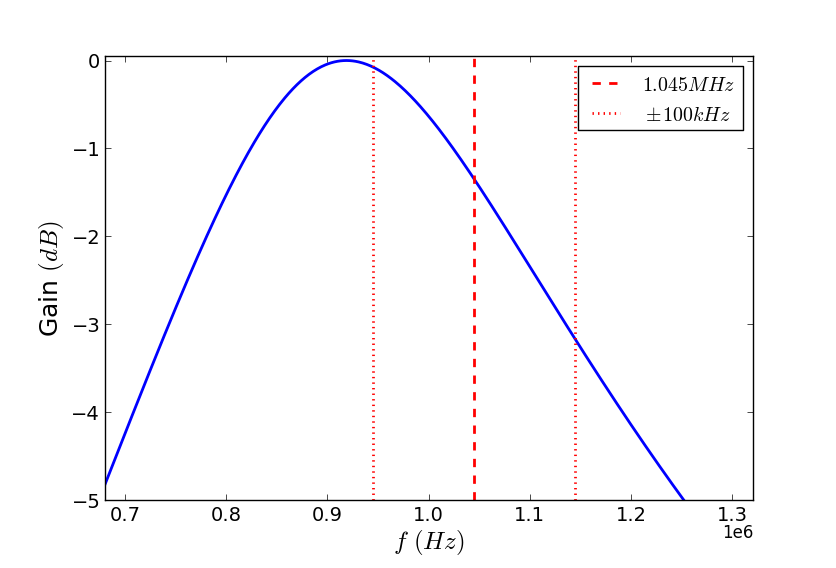
\includegraphics[width=360px]{FM_Reciever_Bandpass_In_dB}
}
\caption{Transfer function of our bandpass filter for $R =13.5\Omega$, $L=1\mu H$, $C=30nF$. This filter has a quality factor of $Q=R\sqrt{\frac{C}{L}}=2.34$ and a bandwidth of $\Delta f_{-3dB}=\frac{f_0}{Q}\approx 390kHz$. The range of carrier wave frequencies of our station lie in the linear region of the transfer function, resulting in an amplitude modulated signal.}
\label{fig:bandpasstransfer}
\end{figure}

To bias the signal properly so that the positive half of the signal would pass through the diode and the negative half would be blocked, we needed to add a DC bias to the signal of $0.6V$. We chose the resistors to be $18k$ (to the power supply) and $2.7k$ (to ground), and had our power supply set to $5.6V$. Using Eq.\ref{eq:voltagedivider}, our bias is $0.72V$, just above our desired voltage.

The low-pass filter needs to be able to smooth out the $1.045MHz$ carrier wave while leaving the underlying audio signal intact. To do this, we want a roll-off frequency somewhere between ~$1MHz$, the carrier frequency, and ~$20kHz$, the upper end of the human audible spectrum. Using Eq.\ref{eq:rolloff}, we choose

\begin{center}
  \begin{tabular}{ c  c }
    C & $1nF$ \\
    R & $1k\Omega$ 
  \end{tabular}
\end{center}
so that we have a roll-off frequency of $f=160kHz$. The transfer function, along with relevant frequencies, are illustrated in Fig.\ref{fig:lowpasstransfer}.
 
\begin{figure}[H]
\center{
  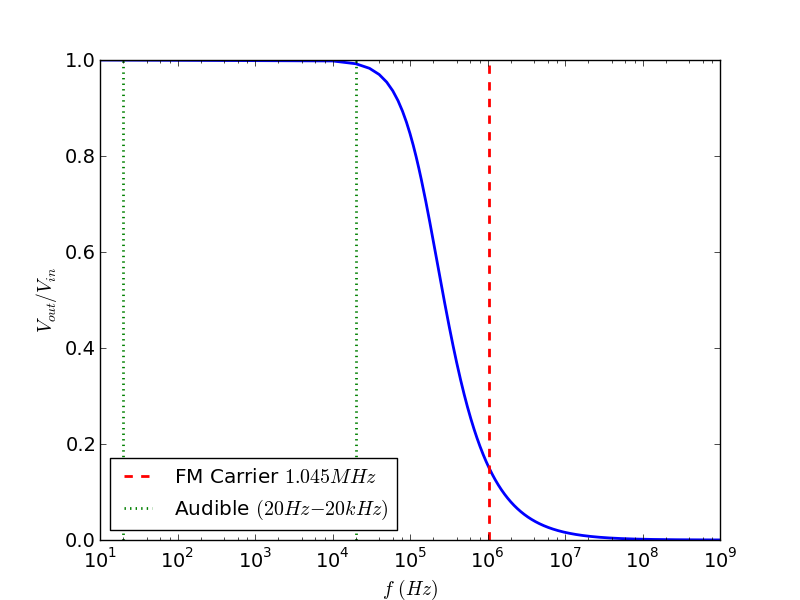
\includegraphics[width=380px]{FM_Reciever_LowPass}
}
\caption{Transfer function of our low-pass filter for $R =1k\Omega$, $C=1nF$, and a roll-off . This filter will essentially average out the high frequencies of the carrier wave (red dotted line) while leaving frequencies in the audible range unattenuated (green dotted lines).}
\label{fig:lowpasstransfer}
\end{figure}

\subsubsection*{Amplifier}
TODO

Next we want to amplify the signal that we have demodulated so that it will be strong enough to be heard through the speakers. The way a NPN transistor works is that if the voltage between the Base and the Emitter, $V_{BE}$ is larger than a certain cut-off value, current will flow from the Collecter through the Emitter. The more current flows through the emitter resistor (the resistor closest to the emitter), the higher the voltage at the emitter will be ($V=IR$). Eventually the emitter voltage becomes large enough that $V_{BE}$ is no longer above the cut-off value and the transistor stops conducting current. Thus, the emitter will be held at a fixed voltage based on what you choose the Base voltage to be (by choosing the bias resistors based on Eq.TODO), minus the cutoff voltage. This is powerful because you can adjust the Base voltage freely and it will force the emitter voltage to follow. Now that you can fix the Emitter voltage (which fixes the current flowing through the collector and emitter), you have fixed the current flowing through the collector resistor and thus have fixed the collector voltage.

Such an amplifier circuit should have a gain of $\frac{R_C}{R_E}$. In our case, we include a capacitor in parallel with the emitter resistor in order to increase the gain for higher frequency signals.

\subsubsection*{Emitter-Follower}
TODO

The purpose of the Emitter-Follower is to provide a buffer between the output of the amplifier and the low impedance load (the speaker). If the follower was not used, the speaker would draw a significant amount of current and voltages in the circuit would drop substantially. The follower has a gain of one, so the signal is unchanged, but by the nature of the transistor the voltage is held steady; instead, more current is sourced from the collector.

\subsection*{Impedance Matching}
It is important to properly terminate cables because of reflections at points where the impedance is mismatched. An improperly terminated line will allow a signal to reflect off of the end and distort the signal at the imput after a short time delay. A signal terminated with a short will see an inverted reflection, and a signal terminated with an open circuit will see an uninverted reflection. The delay between the incoming signal and its reflection is the time it takes for the signal to propogate down the length of the cable and back.

To estimate the length of a very long cable, we sent a square wave signal down it and analyzed the distortion on the scope trace. To estimate the length of the cable, we can analyze the scope trace to determine the time delay, and, estimating the speed of signal propogation in the cable to be $\frac{2}{3}c$, use the relation $l_{cable} \approx \frac{1}{2} \frac{2c}{3} t_{delay}$.

\begin{figure}[H]
\center{
  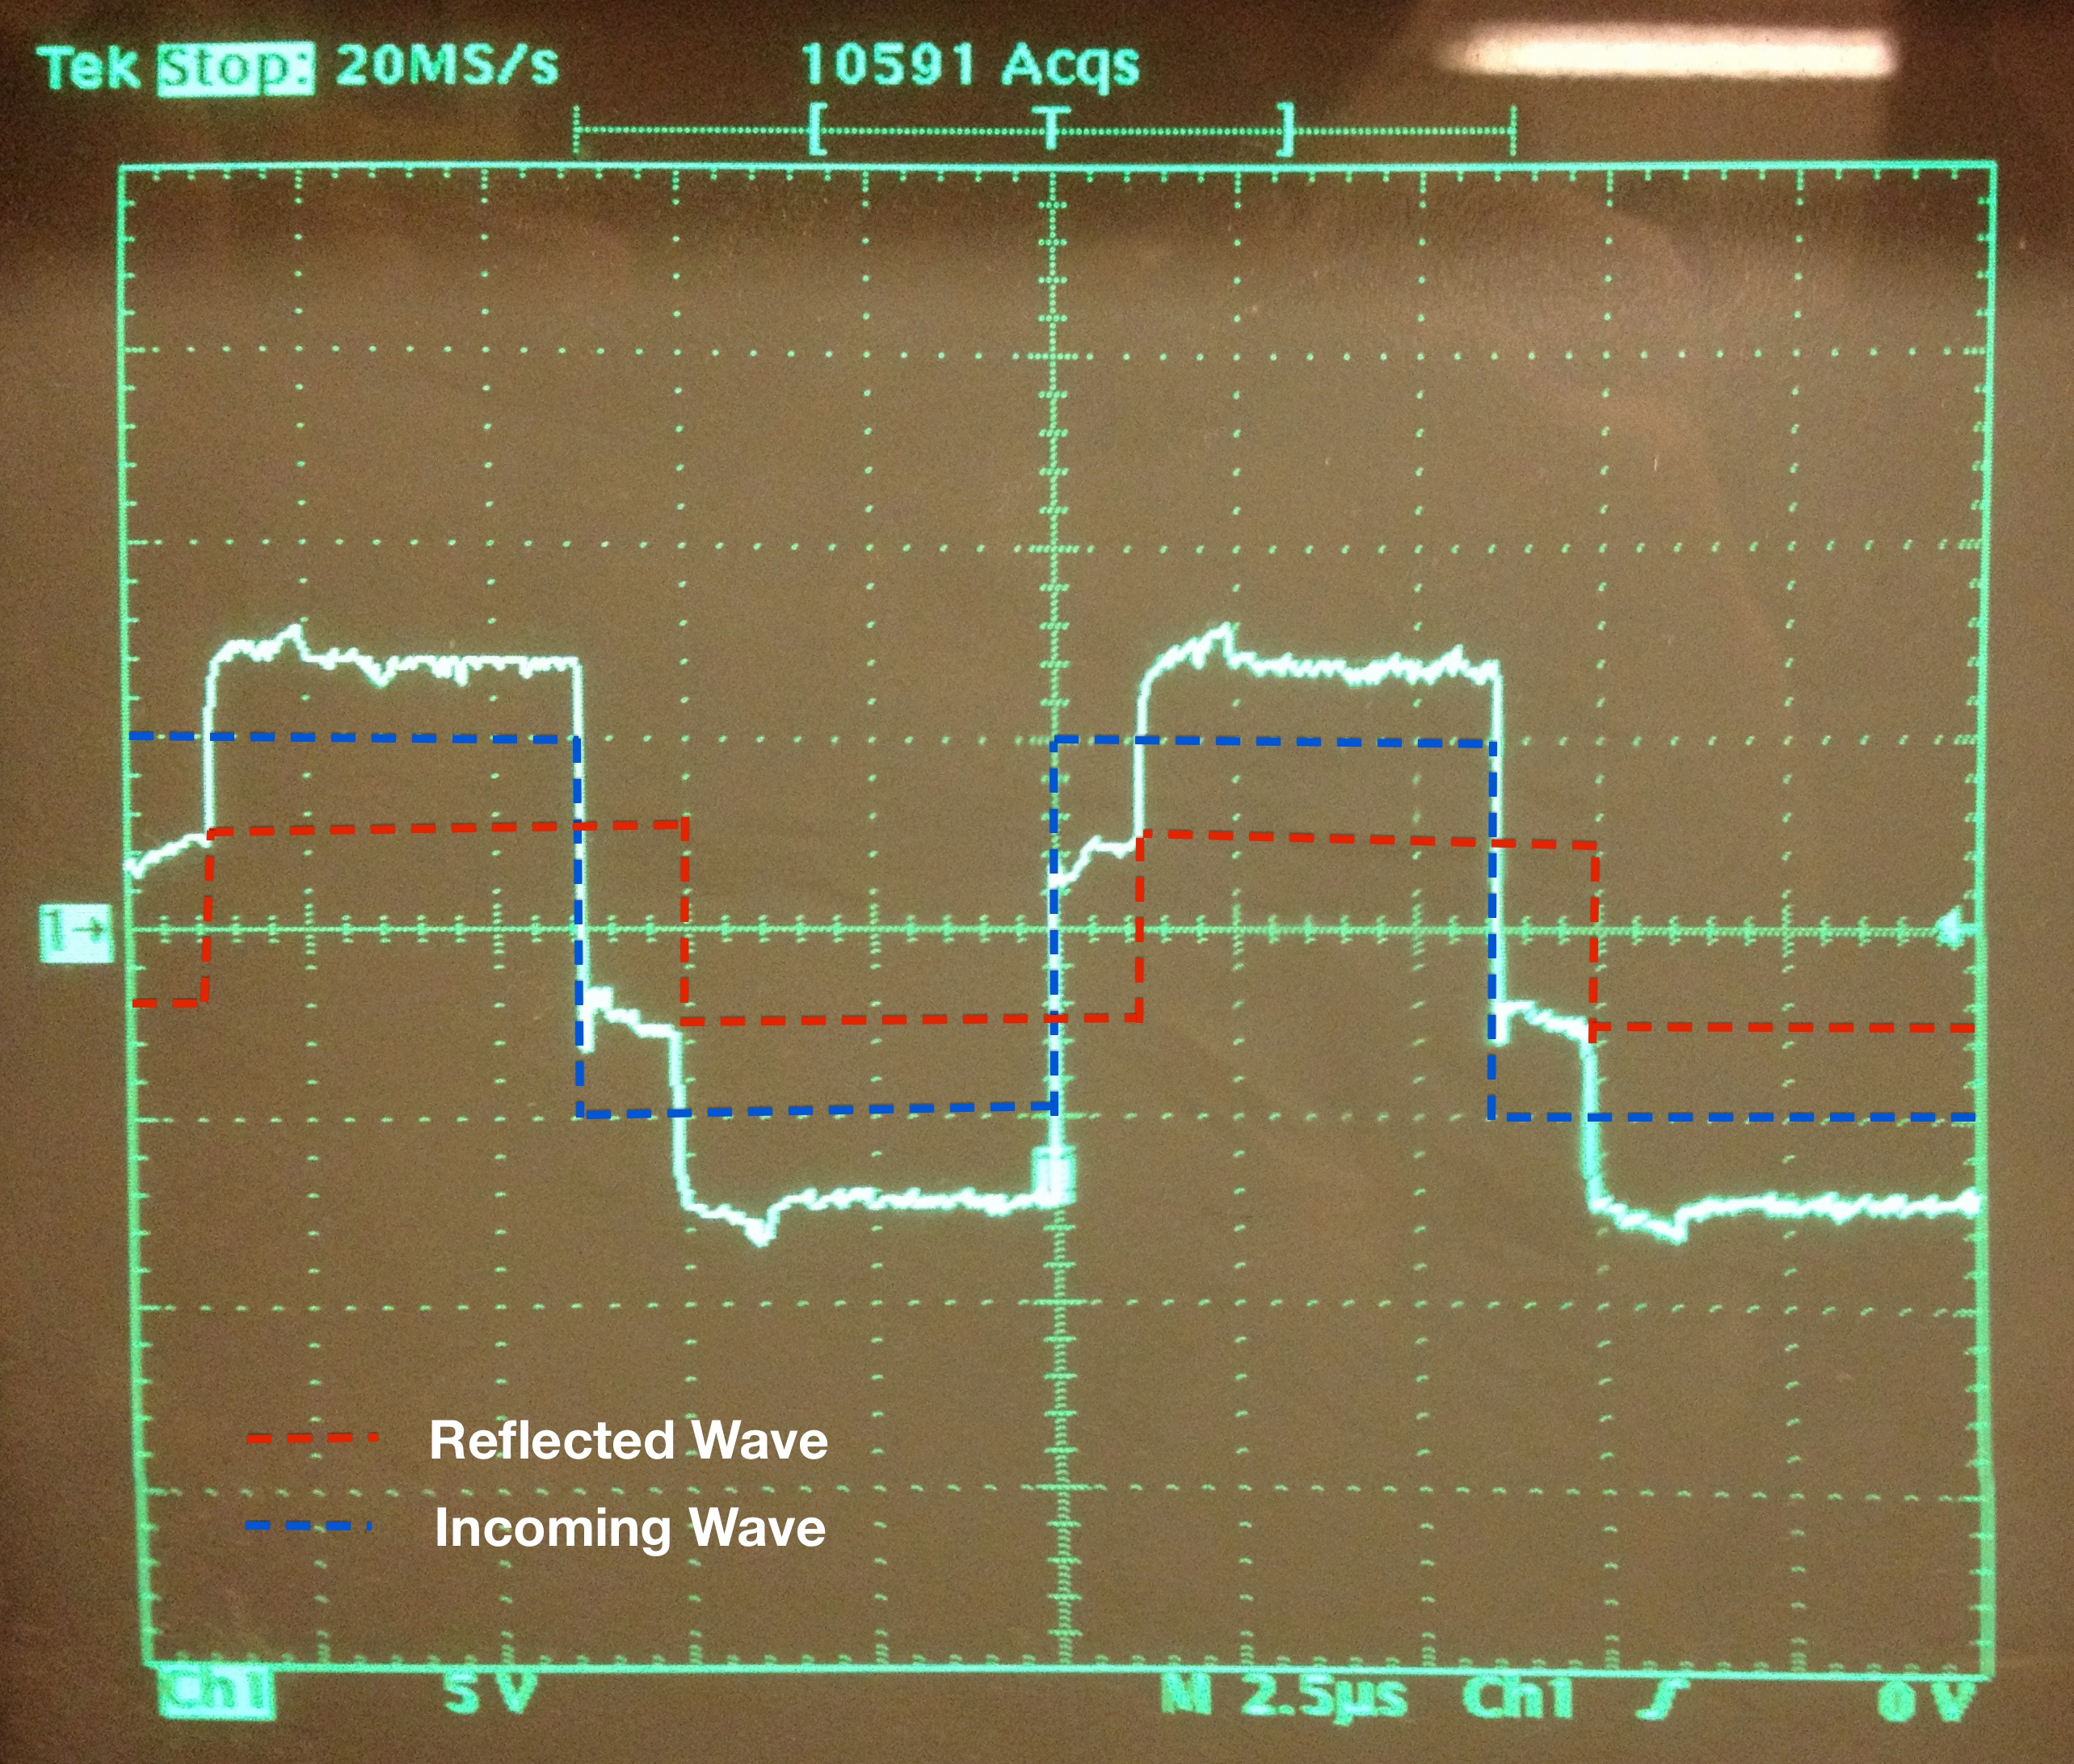
\includegraphics[width=360px]{reflected_signal}
}
\caption[SODUMB]{Scope trace of a $100kHz$ square wave sent down a long cable with no termination. Because the end of the cable is left open, the reflected wave is not inverted and slightly delayed due to the time it takes the signal to travel down the cable and back, and the scope trace shows the sum of the incoming and the reflected waves.}
\label{fig:reflections}
\end{figure}

\subsection*{Measuring Cable Length}
TODO

\subsection*{Noise}
\subsubsection*{Noise Factor}
TODO
\subsubsection*{Central Limit Theorem}
To test and demontstrate the Central Limit Theorem, we will write a program to simulate sampling from random, non-gaussian distributions. By running this a large amount of times, $N$, we will show that the distribution of sampled means is gaussian. To do this I will be interested in the average value of $n=100$ measurements of a random variable---in this case, I will be interested in the average starting value of 100 Blackjack hands\footnote{I will count Aces as 11 unless the sum of the two cards is greater than 21, in which case I count the aces as 1; i.e. the hand AA is worth 12 points).}. By the Law of Large Numbers, the more we make this measurement, the more our results will approach their true distribution; in this case, we hope to see a gaussian distribution.

Additionally, we will demonstrate that the standard deviation on a sampled mean decreases as the inverse square root of the number of samples taken, $n$. For this, we will vary $n$, the number of measurements per sample (i.e., I will determine the distribution of the average starting value of $n$ Blackjack hands, for $n=5,10,50,$ and $100$). By plotting histograms of the results, we should be able to see that the width fo the distribution decreases for larger $n$, and if we find the standard deviation at many values of $n$ we should be able to fit a power law to it and verify the CLT, that $\sigma \propto n^{-1/2}$.

The code I wrote and used can be found in my github respository at

 http://github.com/kevinyu/astro121.git

\section*{Results}
\subsection*{Demodulator Bandpass Filter}
Choosing component values in our bandpass filter gave us a little trouble, due to lost factors of $2\pi$ here and there. Every component value is important here: if the resonant frequency is too low, or the bandwidth too narrow (resistor too large), the carrier wave frequencies may fall too far down the response curve and the signal may be attenuated too severely. Convesely, if the resonant frequency is too close to the carrier wave center frequency, or the bandwidth too wide (resistor too small), there may not be enough difference in attenuation across the span of FM frequencies to make a good AM signal. The values that we selected in the Methods section worked well and produced a good AM signal that we were able to extract and ultimately hear in the speaker.  
\subsection*{Demodulator Biasing}
One issue we had at first was a boring, flat, DC output coming out of the low-pass at the end of the demodulator, rather than the desired signal. After a bit of confusion, we realized it was due to choosing poor values for our biasing resistors. Originally, we had chosen them both to be the same value; Because it is a voltage divider, the bias would have been one half of the power supply voltage, or $2.8V$. As we know, from the Method section, we needed the diode to pass the positive half of the signal but block the negative half of the signal. However, because here our bias was $2.8V$, much greater than the diode ``on" voltage of $0.6V$, the diode will pretty much \textit{always be conducting}. Thus, the low-pass filter averaged out the AM signal entirely and the amplitude information was lost. To fix this, we chose biasing resistors such that the bias voltage would be much closer to $0.6V$, and found that the demodulator was then successful.

\subsection*{Length of the Cable}
To approximate the length of the cable in the lab, we use the method described in the Method section and Eq.\ref{eq:cablelength}. The scope trace, with the sum of the incoming wave and reflected wave, can be seen in Fig.\ref{fig:reflections}. As we can see on the scope trace, the reflected wave is delayed by about $1.2\mu s$, and thus the cable length is (assuming the speed of signal propogation in the cable is $\frac{2}{3}c$):
\begin{eqnarray}
l_{cable} \approx 120m \nonumber
\end{eqnarray}
This is a reasonable result, and is only as accurate as the approximation that $c_{cable} \approx \frac{2}{3}c$.

\subsection*{Impedance of the Cable}
To estimate the impedance of the cable, we will try terminating it with different valued resistors until we do not see any reflections. When terminating the cable with a $10\Omega$ resistor, we saw that the reflection was inverted. We had gone too far. We took this to mean that the impedance of the cable was somewhere between $10\Omega$ and $\infty\Omega$, which really narrowed it down for us. Luckily, our next choice of $56\Omega$ turned out to be close enough, and we saw a very nice trace of a square wave on the oscilloscope with no distorting reflections.
\begin{eqnarray}
Z_{cable} \approx 56\Omega \nonumber
\end{eqnarray}

\subsection*{Noise Figure and Y-Factor}
TODO

\subsection*{Central Limit Theorem Results}
In Fig.\ref{fig:approachgaussian}, we can see that the distribution of a sampled mean is approximately gaussian. By the Law of Large Numbers, the larger we make the value of $N$ the closer our measurements will approximate their true distribution. For the figure, we measure the average starting value of $n=100$ blackjack hands. As you can see in the figure, at large values of $N$ our results show that the distribution of a sampled mean is approximately gaussian. This is true even though the distribution of a single measurement is not gaussian, the distribution of the mean of multiple measurements is.

\begin{figure}[H]
\center{
  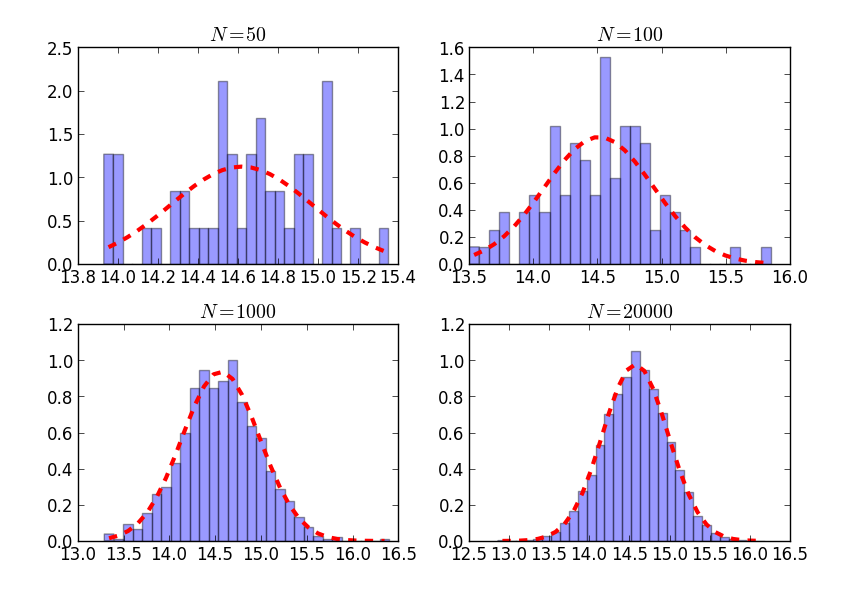
\includegraphics[width=360px]{Blackjack_Gaussian}
}
\caption[SODUMB]{Distribution of the average starting value of $n=100$ blackjack hands. At large $N$, the results should approach their true distribution. The dotted red line is a fitted gaussian to the data.}
\label{fig:approachgaussian}
\end{figure}
To demonstrate the standard deviation's $\frac{1}{\sqrt{n}}$ dependence, I sampled the average value of $n$ randomly chosen numbers between 0 and 10 (inclusive) for values of $n$ ranging from 2 to 10000. For each value of $n$, I will record the standard deviation of $N=20$ measurements of the mean.
\begin{figure}[H]
\center{
  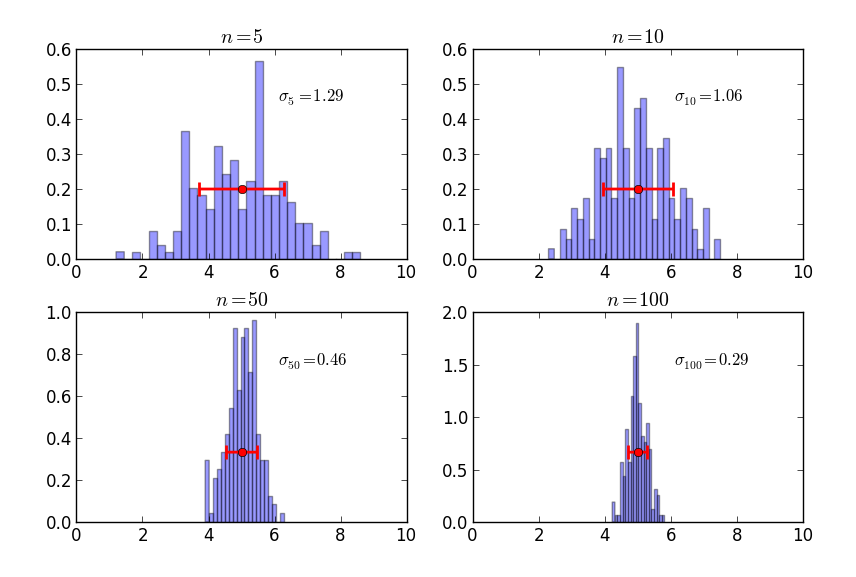
\includegraphics[width=360px]{CLT_n_scaling}
}
\caption[SODUMB]{The standard deviation of $N=20$ measurements of samples of size $n$, for $n=5,10,50,100$. As you can see, the width of the distribution decreases as $n$ increases. Note that all four histograms have the same scale on the x-axis.}
\label{fig:n_scaling}
\end{figure}
\begin{figure}[H]
\center{
  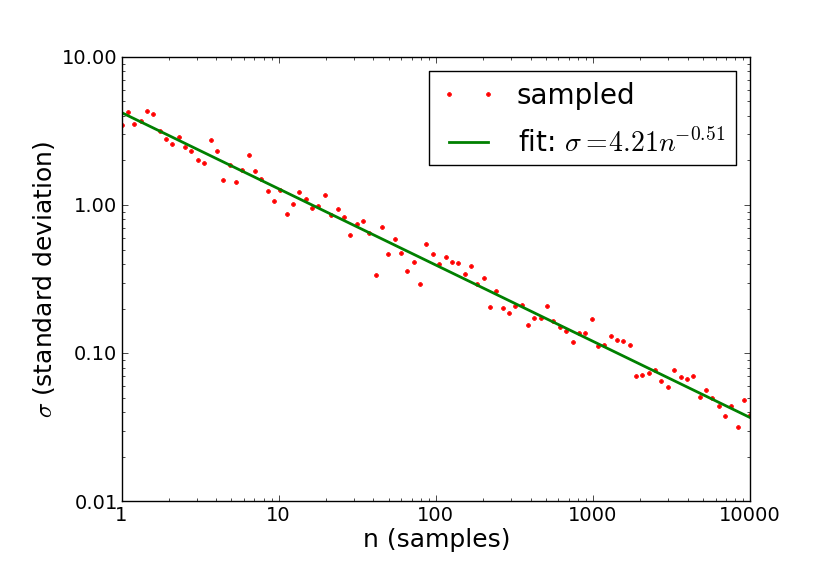
\includegraphics[width=360px]{CLT_sigma_vs_n}
}
\caption[SODUMB]{The relationship between the sampled standard deviation, $\sigma$, and the number of samples in each measurement, $n$, visualized on a log-log plot. It is clear that the data approximately follows a $n^{-1/2}$ rule, as a least-squares fit returned a power relationship of $\sigma \propto n^{-0.51\pm0.02}$.}
\label{fig:n_scaling2}
\end{figure}


\section*{Conclusion}

\section*{Acknowledgement}
Thanks to Jeff Lievense and Maissa Salama for working hard in getting through this lab with me. Thanks to the lab instructors---Prof. Aaron Parsons, Karto, and Baylee---for making the lab possible to complete, despite the pain it has caused.
Plots were done in Python using the Numpy and Matplotlib libraries.
Voltage divider image shamelessly stolen from the lab manual.
Circuit diagrams created in LTSpice.

\begin{thebibliography}{1}

\end{thebibliography}

\end{document}